\section{Additional Qualitative and Benchmark Results}
\label{app:additional_results}



\subsection{Qualitative Analysis for Zero-Shot Cross-Embodiment Experiments}
We present additional qualitative comparisons of all baseline policies under zero-shot embodiment transfer, complementing the results in Section~\ref{subsec:zero_shot}. 
OpenVLA~\cite{kim2024openvlaopensourcevisionlanguageactionmodel}, MolmoAct~\cite{lee2025molmoactactionreasoningmodels}, and $\pi_{0.5}$-Base \cite{intelligence2025pi05visionlanguageactionmodelopenworld} consistently fail to produce meaningful motions across all robot platforms. 
X-VLA~\cite{zheng2025xvlasoftpromptedtransformerscalable} generates smooth trajectories and occasionally approaches target objects on the DROID and Custom Franka setups; however, it never achieves accurate gripper–object alignment required for successful manipulation.

The $\pi_{0}$-replicated baseline exhibits highly imprecise end-effector control. For instance, in the \emph{Tissue} task on the YAM robot, it frequently overshoots the target and grasps the tissue box rather than the tissue itself. In contrast, $\pi_{0.5}$-replicated generally produces smoother and more directionally reasonable motions, but still lacks the spatial precision required for reliable grasping and successful task completion. Across the Custom Franka and Kinova robots, both baselines similarly exhibit imprecise motions, suggesting limited ability to infer accurate control actions under embodiment shift. These failure modes are consistent across all evaluated embodiments. An example rollout is shown in Fig.~\ref{fig:baseline-rollout-visualization}.

\begin{figure*}[h]
    \centering
    \includegraphics[width=\linewidth]{figures/appendix/fig12_baseline_rollout.pdf}
   \caption{\textbf{Example baseline rollout failures on the Sort task (YAM robot).} 
    Both $\pi_{0}$-replicated and $\pi_{0.5}$-replicated exhibit imprecise end-effector control, moving directly toward the basket without first grasping any objects. 
    In contrast, LAP-3B successfully completes the task under similar initial conditions. 
    Open-sourced VLA baselines are omitted as they do not generate meaningful or safe control actions in this setting.}
    \label{fig:baseline-rollout-visualization}
\end{figure*}
\vspace{-5pt}

% \begin{figure}[h]
%     \centering
%     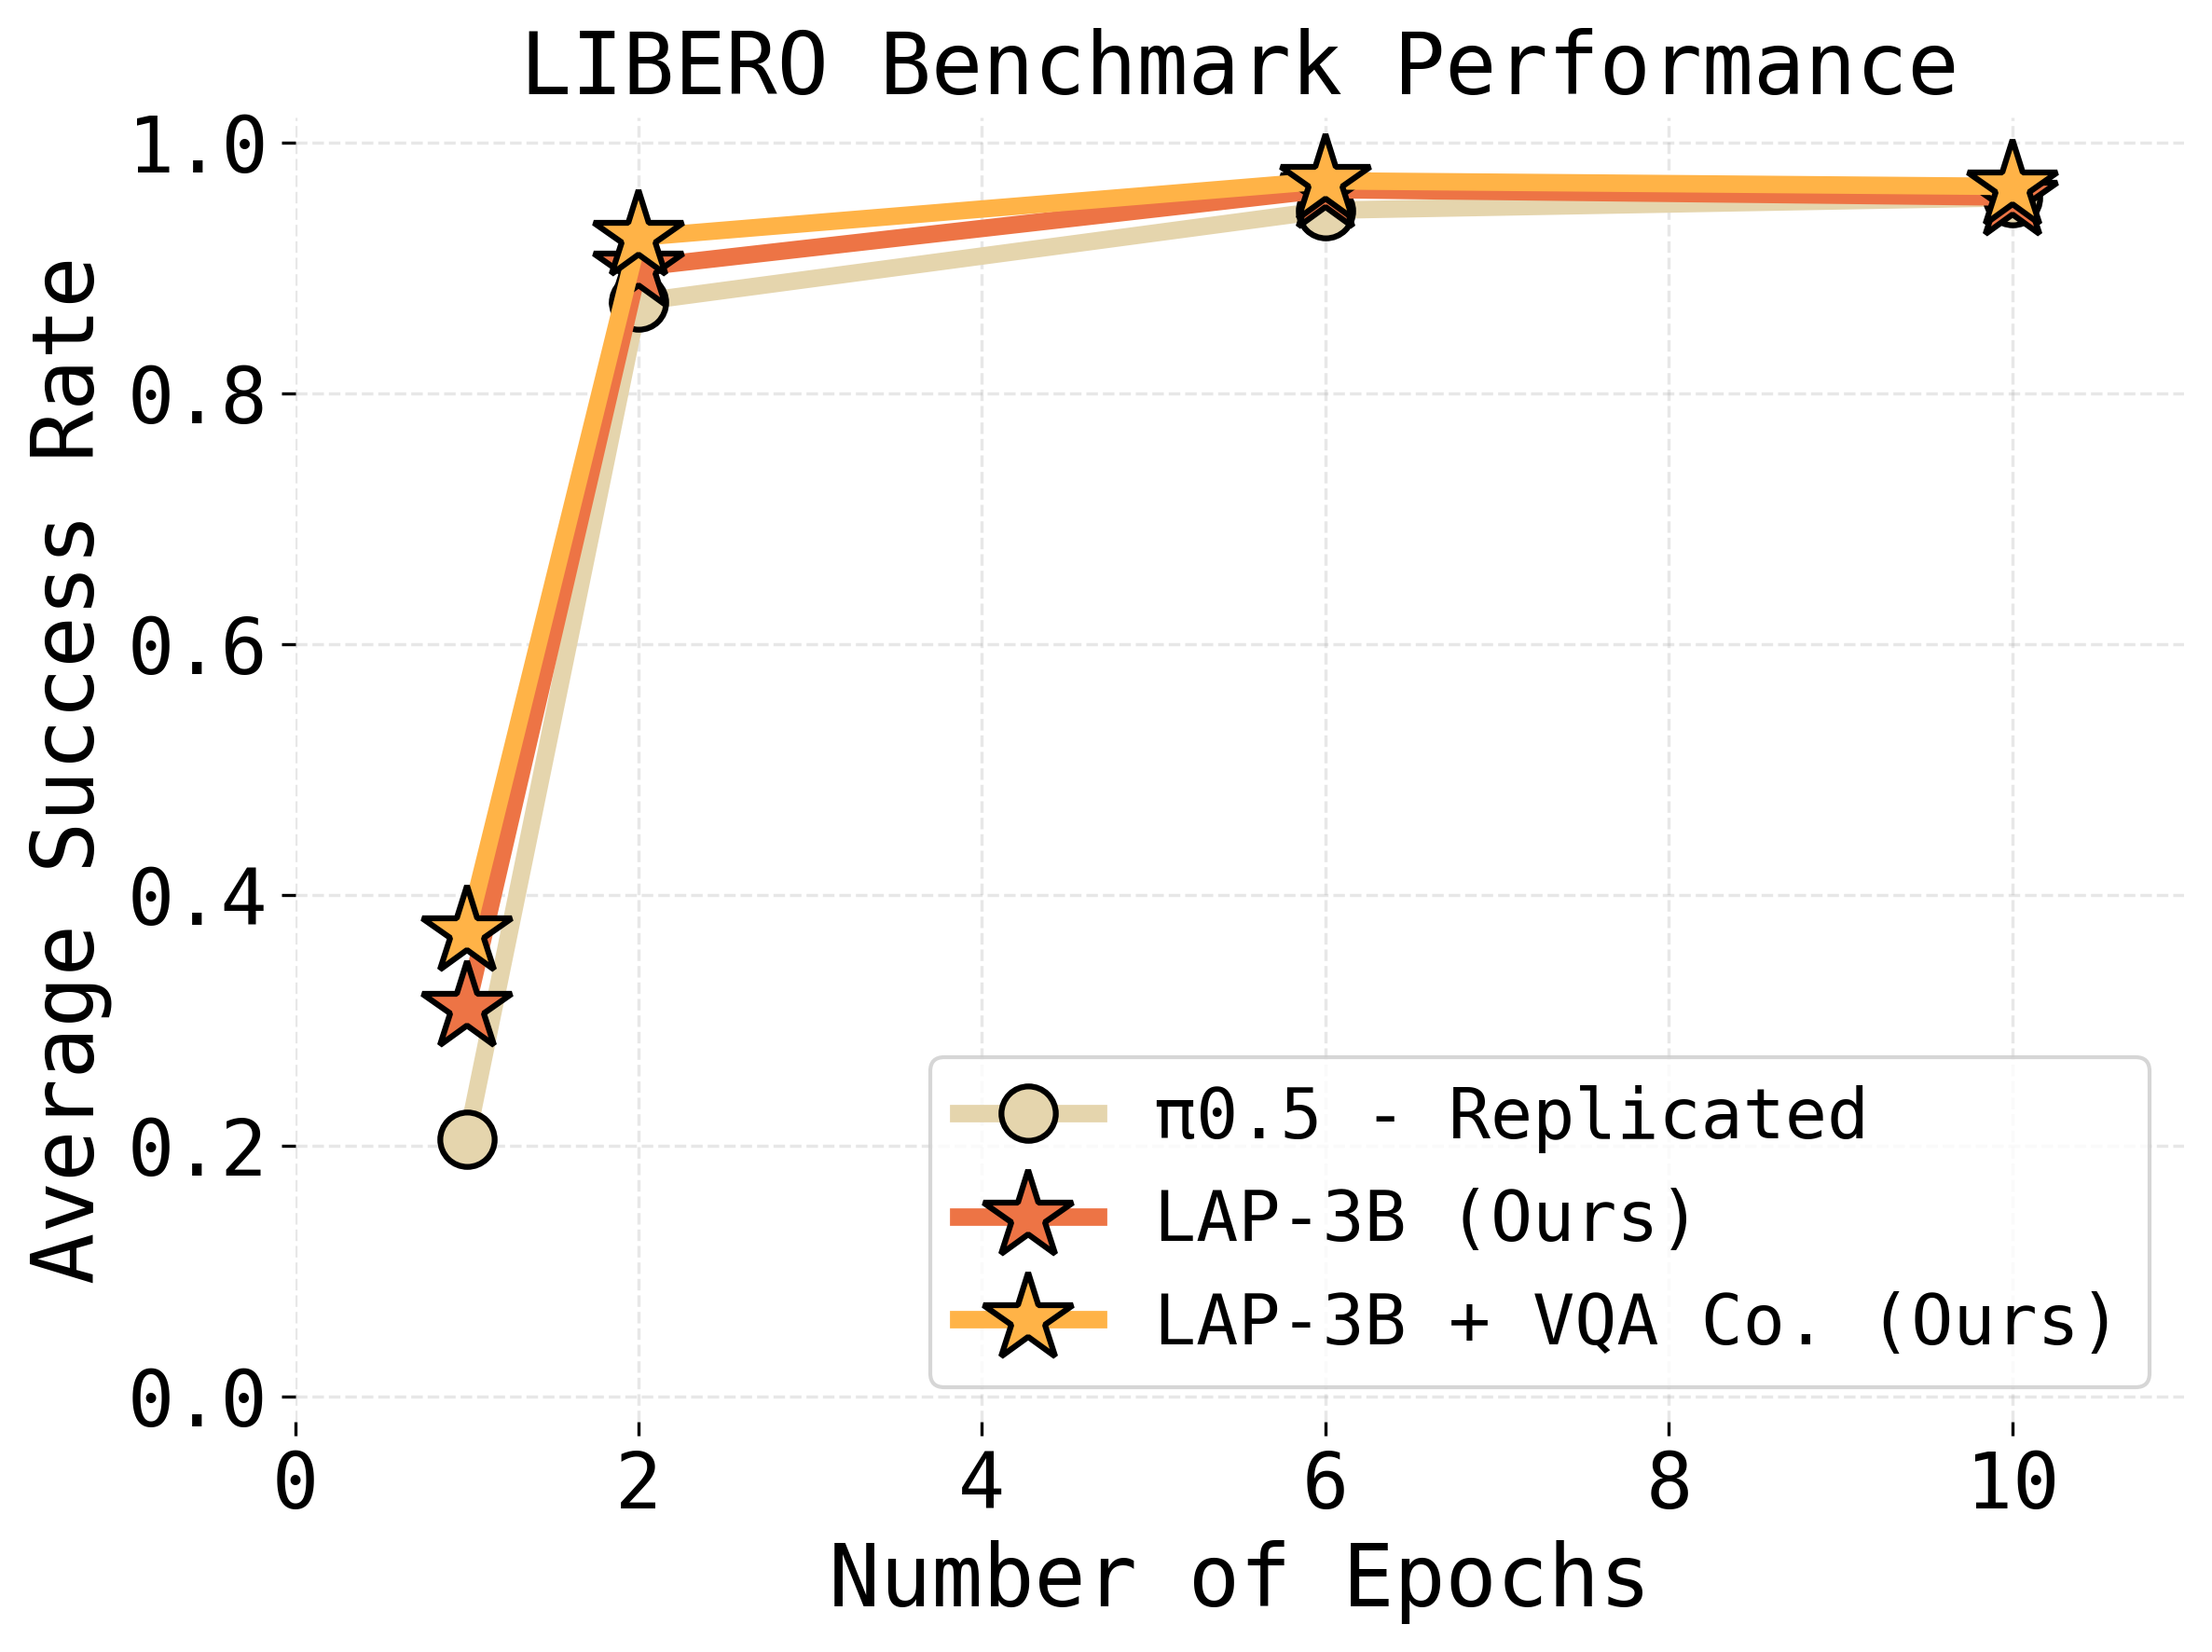
\includegraphics[width=\linewidth]{figures/appendix/fig14_libero_cotrain.png}
%     \caption{\textbf{Compute efficiency on the LIBERO benchmark.} Co-training with VQA data significantly accelerates convergence, enabling \textsc{LAP-3B}+VQA Co-training to achieve high success rates in fewer gradient steps than \textsc{LAP-3B}. For clarity, we report only the strongest replicated baseline ($\pi_{0.5}$-replicated).}
%     \vspace{-8pt}
%     \label{fig:libero-cotraining}
% \end{figure}


\begin{figure*}[b]
    \centering
    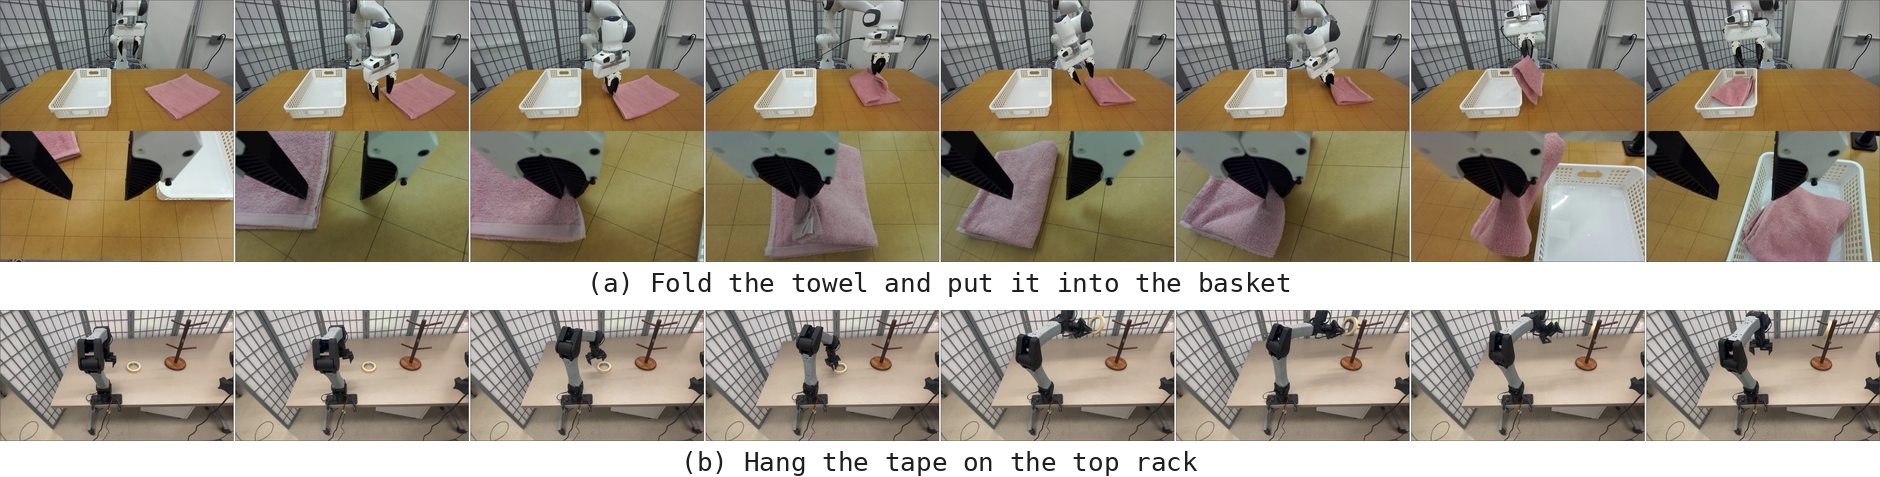
\includegraphics[width=\linewidth]{figures/appendix/fig11_finetune_rollout.png}
    \caption{\textbf{Fine-tuning evaluation rollout visualizations.} Example observations from the camera views used for policy evaluation across different robot embodiments and tasks, shown from left to right.}
    \label{fig:finetuning-rollout-visualization}
\end{figure*}
\vspace{2pt}


\begin{table}[!h]
\centering
\footnotesize
\setlength{\tabcolsep}{4pt}
\caption{LIBERO benchmark results comparing LAP-3B with other state-of-the-art VLAs. Each data point corresponds to an average over 500 trials. Best per column is bolded. Rank is based on Avg. performance (higher is better).}
\begin{tabular}{l c c c c c c}
\toprule
Method & Spatial & Object & Goal & LIBERO-10 & Avg. & Rank \\
\midrule

TraceVLA \cite{zheng2025tracevlavisualtraceprompting} 
& 84.6 & 85.2 & 75.1 & 54.1 & 74.8 & 13 \\

X-VLA \cite{zheng2025xvlasoftpromptedtransformerscalable} 
& 98.2 & 98.6 & 97.8 & \textbf{97.6} & \textbf{98.1} & 1 \\

Octo \cite{octomodelteam2024octoopensourcegeneralistrobot} 
& 78.9 & 85.7 & 84.6 & 51.1 & 75.1 & 12 \\

UniAct \cite{zheng2025universalactionsenhancedembodied} 
& 77.0 & 87.0 & 77.0 & 70.0 & 77.8 & 11 \\

GR00T-N1 \cite{nvidia2025gr00tn1openfoundation} 
& 94.4 & 97.6 & 93.0 & 90.6 & 93.9 & 8 \\

OpenVLA \cite{kim2024openvlaopensourcevisionlanguageactionmodel} 
& 84.7 & 88.4 & 79.2 & 53.7 & 76.5 & 10 \\

OpenVLA-OFT \cite{kim2025finetuningvisionlanguageactionmodelsoptimizing} 
& 97.6 & 98.4 & 97.9 & 94.5 & 97.1 & 3 \\

UniVLA \cite{bu2025univlalearningacttaskcentric} 
& 95.4 & 98.8 & 93.6 & 94.0 & 95.4 & 6 \\

$\pi_0$ \cite{black2024pi0visionlanguageactionflowmodel} 
& 96.8 & 98.8 & 95.8 & 85.2 & 94.2 & 7 \\

$\pi_{0.5}$ \cite{intelligence2025pi05visionlanguageactionmodelopenworld} 
& 98.8 & 98.2 & 98.0 & 92.4 & 96.9 & 4 \\

VLA-0 \cite{goyal2025vla0buildingstateoftheartvlas} 
& 97.0 & 97.8 & 96.2 & 87.6 & 94.7 & 9 \\

% \midrule
% \multicolumn{7}{l}{\underline{\textit{Replicated / Oracle Baselines}}} \\

% $\pi_0$-replicated 
% & 96.8 & 98.4 & 95.6 & 87.2 & 94.5 & -- \\

% $\pi_{0.5}$-replicated 
% & 96.0 & \textbf{99.6} & 97.8 & 90.8 & 96.1 & -- \\

% \textcolor{gray}{$\pi_{0.5}$-Oracle} 
% & \textcolor{gray}{\textbf{99.8}} 
% & \textcolor{gray}{98.6} 
% & \textcolor{gray}{\textbf{99.2}} 
% & \textcolor{gray}{\textbf{96.0}} 
% & \textcolor{gray}{\textbf{98.4}} 
% & -- \\

\midrule
\textbf{\textsc{LAP-3B}} 
& 98.2 & \textbf{99.0} & \textbf{98.8} & 91.2 & 96.8 & 5 \\

\textbf{\textsc{LAP-3B}+ VQA Co.} 
& \textbf{99.0} & \textbf{99.0} & 97.2 & 93.4 & 97.2 & 2 \\

\bottomrule
\end{tabular}
\label{tab:libero_full}
\end{table}




\subsection{Full Results for the LIBERO Benchmark}
\begin{wrapfigure}{r}{0.4\textwidth}
    \centering
    \vspace{-20pt}
    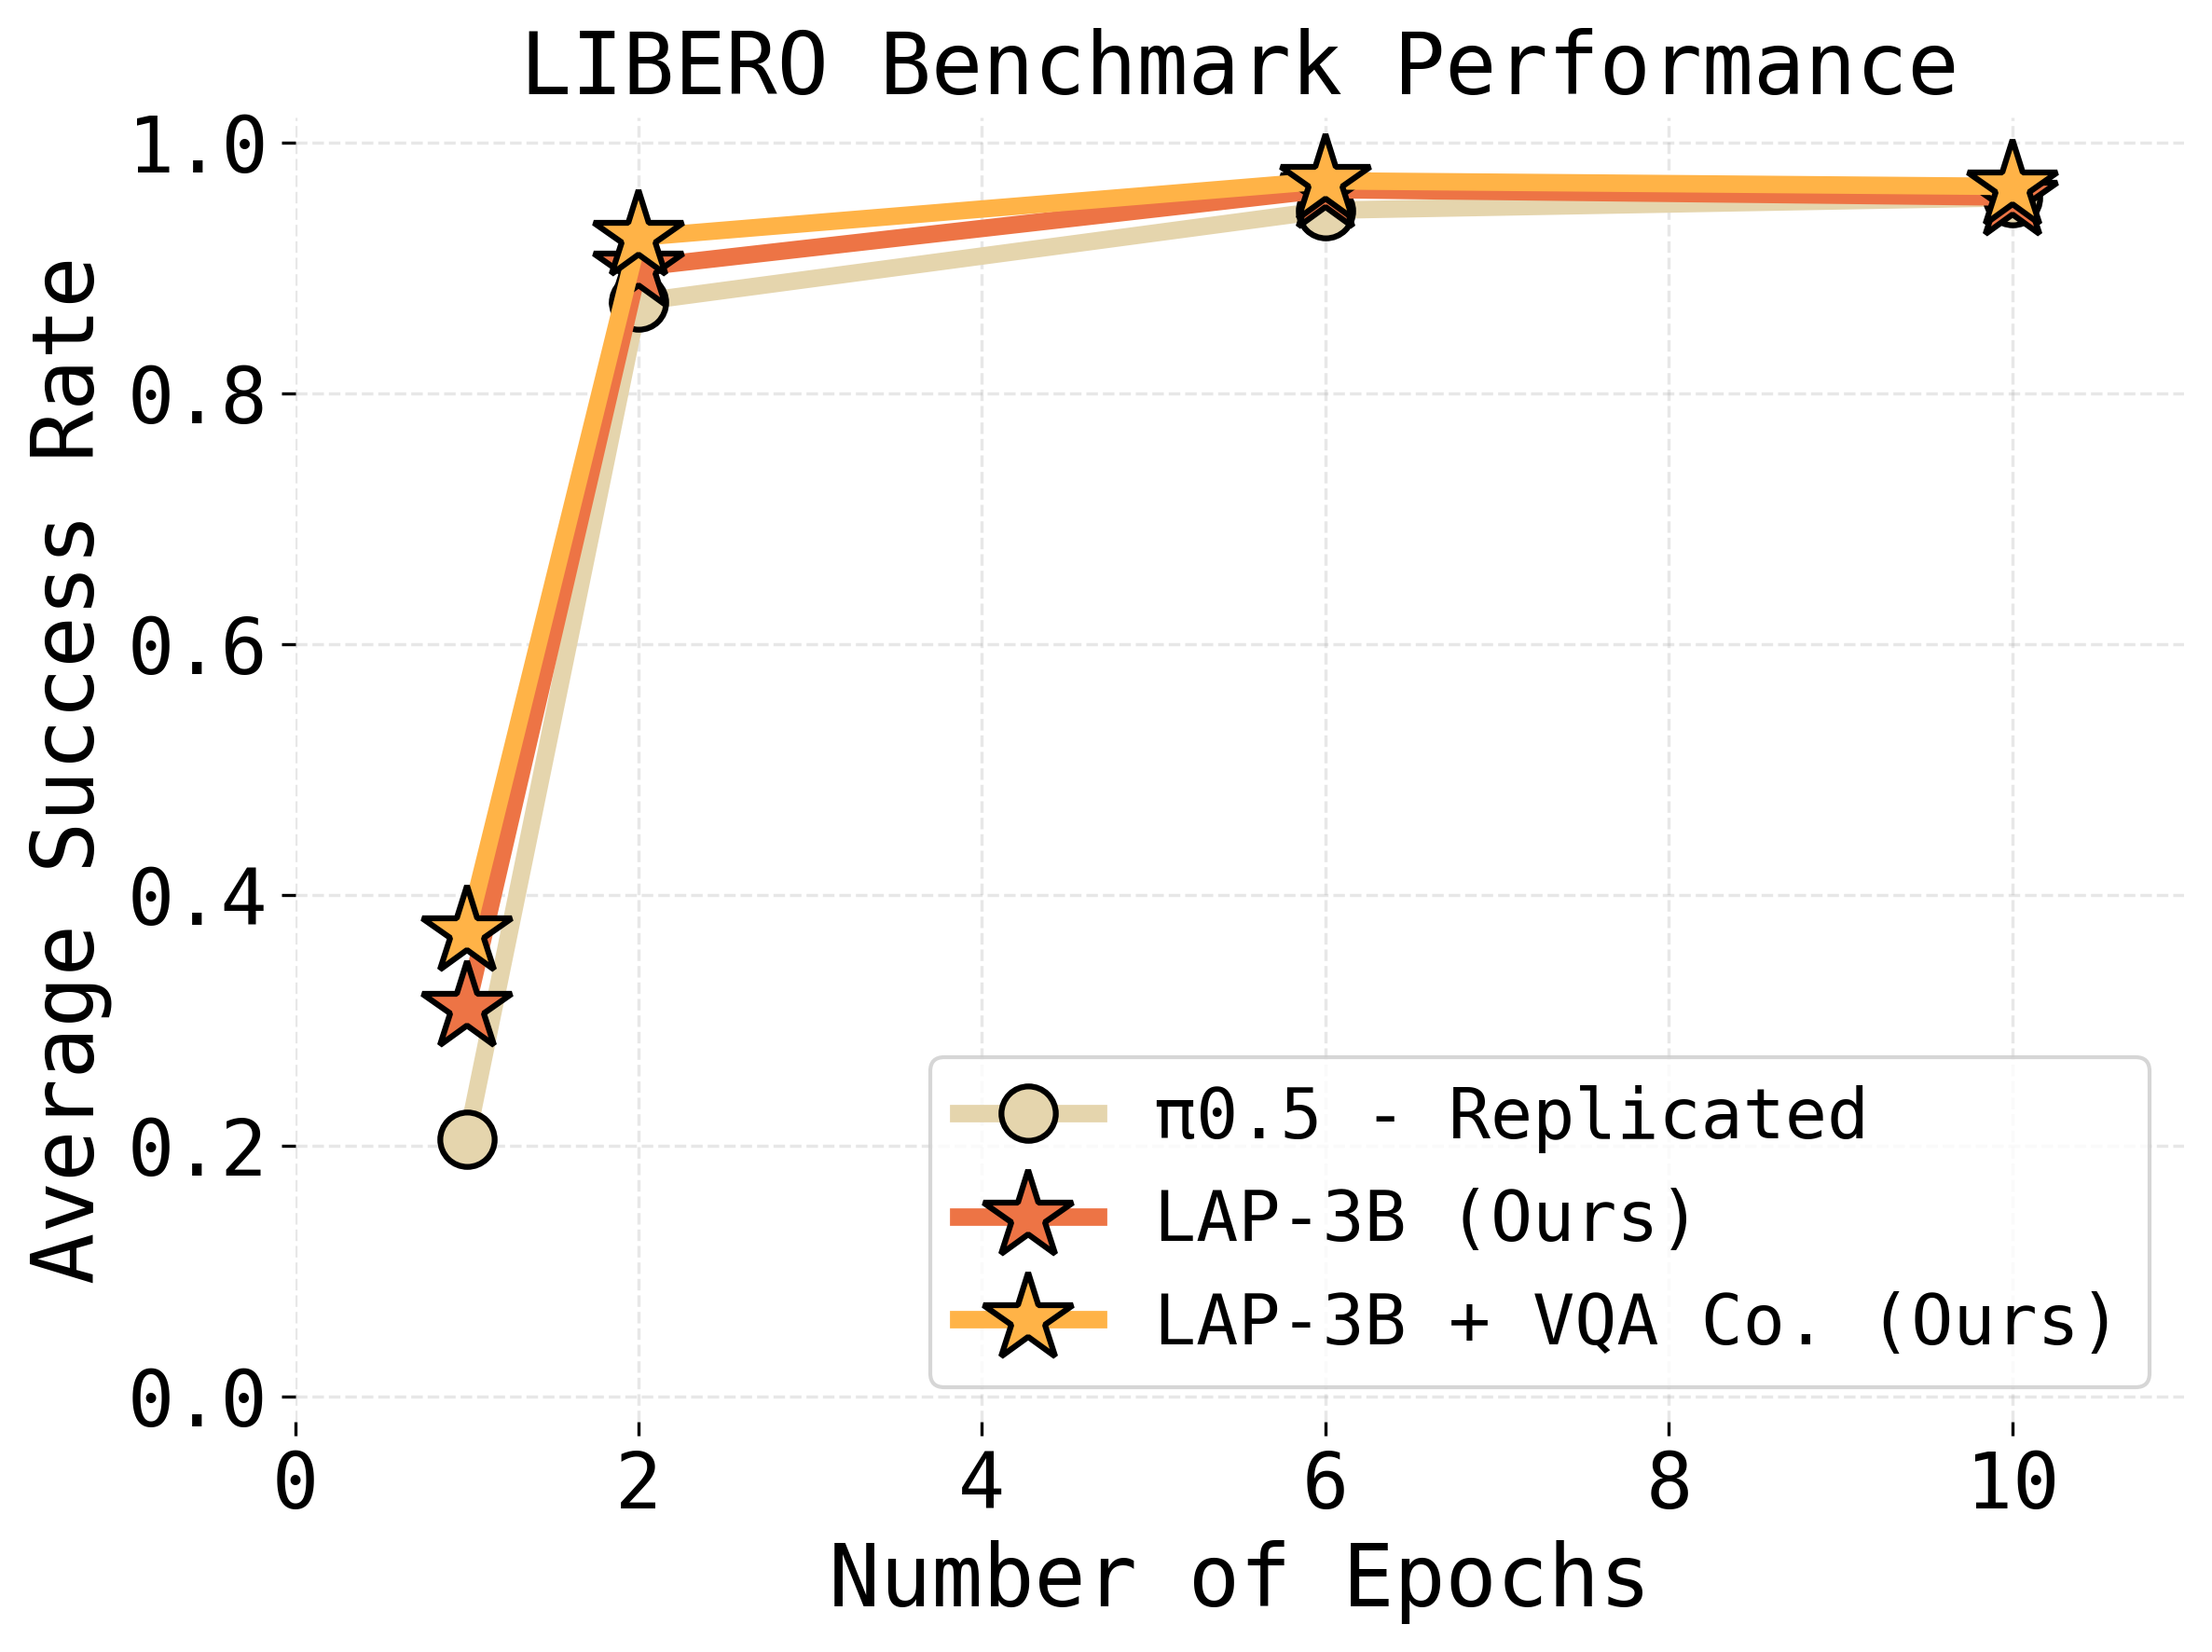
\includegraphics[width=0.4\textwidth]{figures/appendix/fig14_libero_cotrain.png}
    \captionsetup{skip=2pt}
    \caption{\textbf{Compute efficiency on LIBERO.} Co-training with VQA data significantly accelerates convergence, enabling \textsc{LAP-3B}+VQA Co-training to reach high success rates in fewer gradient steps. For clarity, we report only the strongest baseline ($\pi_{0.5}$-replicated).}
    \vspace{-1cm}
    \label{fig:libero-cotraining}
\end{wrapfigure}
Table~\ref{tab:libero_full} reports the complete LIBERO benchmark results, including additional open-source VLA baselines not shown in the main paper, and further confirms the consistent performance gains of \textsc{LAP-3B} across task families and all three task suites. \textsc{LAP-3B}+VQA Co. denotes the policy co-trained with VQA data as described in Section~\ref{sec:experiments}. Its improved performance over \textsc{LAP-3B} alone further underscores the effectiveness of VQA co-training. Moreover, the co-trained checkpoint substantially improves fine-tuning efficiency on LIBERO, achieving stronger performance with the same gradient steps, as shown in Fig.~\ref{fig:libero-cotraining}.


\subsection{Real-Robot Rollouts}
We further provide extended qualitative rollout visualizations across all embodiments and tasks for fine-tuning evaluation in Fig.\ref{fig:finetuning-rollout-visualization} and zero-shot evaluation in Fig.~\ref{fig:zeroshot-rollout-visualization}. 
Each panel corresponds to the camera views used during policy execution. 


\section{Implementation Details}
\label{app:implementation_details}

\subsection{Robot Platforms} 
We evaluate \textsc{LAP-3B} across four robot embodiments that differ in kinematics, sensing configurations, and control interfaces:
\begin{itemize}
\item \textbf{DROID}: a seen embodiment during pre-training, comprising a 7-DoF arm with both external and wrist-mounted cameras.
\item \textbf{Custom Franka}: an unseen 7-DoF arm with external and wrist-mounted cameras, featuring a novel gripper and wrist camera mounting that differ from Franka robots observed during training.
\item \textbf{YAM}: an unseen 6-DoF arm with a single external camera.
\item \textbf{Kinova}: an unseen 7-DoF arm with external and wrist-mounted cameras.
\end{itemize}

For fine-tuning, we use joint-space actions on YAM to enable more precise low-level control, while all other robots are controlled using end-effector pose actions.




\subsection{Training Hyperparameters} 
\begin{wraptable}{r}{0.4\textwidth}
    \centering
    \small
    % \vspace{-10pt}
    \vspace{-1.2cm}
    \caption{Training Hyperparameters for LAP-3B.}
    \label{tab:hyperparams}
    \renewcommand{\arraystretch}{1.15}
    \begin{tabular}{l c}
    \toprule
    \textbf{Hyperparameter} & \textbf{Value} \\
    \midrule
    Batch size & 2048 \\
    Learning rate & $1 \times 10^{-4}$ \\
    Warmup steps & 5000 \\
    EMA start step & 5000 \\
    EMA decay & 0.999 \\
    Action horizon & 16 \\
    Adam $(\beta_1, \beta_2)$ & $(0.9,\ 0.95)$ \\
    Gradient clipping norm & 1.0 \\
    Weight decay & $1 \times 10^{-4}$ \\
    \bottomrule
    \end{tabular}
    \vspace{-8pt}
\end{wraptable}
The overall training objective is:
\[
\mathcal{L} = \mathcal{L}_{\text{flow}} + \lambda \mathcal{L}_{\text{CE}}.
\]

We use $\lambda=0.8$ during pre-training and $\lambda=0.4$ during fine-tuning. Other hyper-parameters is shown in Table.\ref{tab:hyperparams}. We set $\lambda<1$ during pre-training to slightly downweight the language-action loss, as it converges substantially faster than the diffusion-based action expert. This balancing prevents the faster language-action objective from dominating optimization and encourages both components to learn at comparable rates.


\subsection{Baseline Implementations}
For all replicated baselines ($\pi_{0.5}$-replicated, $\pi_{0}$-replicated, and VLA-0-replicated), we carefully tune hyperparameters and select the best-performing checkpoints based on preliminary real-robot validation runs. 
Across all baselines, we sweep the learning rate over $\{1\times10^{-4}, 5\times10^{-5}\}$ and the batch size over $\{1024, 2048\}$. 
For $\pi_{0.5}$-replicated, we additionally sweep the cross entropy loss weight of the FAST tokens over $\{0.1, 0.4, 0.6, 0.8\}$ and the action horizon over $\{16, 32\}$.

% \begin{wraptable}{r}{0.4\textwidth}
%     \centering
%     \small
%     \vspace{-10pt}
%     \caption{Training Hyperparameters for LAP-3B.}
%     \label{tab:hyperparams}
%     \renewcommand{\arraystretch}{1.15}
%     \begin{tabular}{l c}
%     \toprule
%     \textbf{Hyperparameter} & \textbf{Value} \\
%     \midrule
%     Batch size & 2048 \\
%     Learning rate & $1 \times 10^{-4}$ \\
%     Warmup steps & 5000 \\
%     EMA start step & 5000 \\
%     EMA decay & 0.999 \\
%     Action horizon & 16 \\
%     Adam $(\beta_1, \beta_2)$ & $(0.9,\ 0.95)$ \\
%     Gradient clipping norm & 1.0 \\
%     Weight decay & $1 \times 10^{-4}$ \\
%     \bottomrule
%     \end{tabular}
%     \vspace{-8pt}
% \end{wraptable}

Unless otherwise specified, the final hyperparameters used for all replicated baselines are a batch size of $2048$, learning rate of $1\times10^{-4}$, action horizon of $16$, and loss weight of $\lambda=0.6$.

Beyond these explicitly tuned parameters, all replicated baselines share the same design choices as our method, including identical network architectures, data mixtures, sampling strategies, and optimization settings. 
All remaining hyper-parameters follow those listed in Table~\ref{tab:hyperparams}.

For $\pi_{0}$-replicated, we directly follow the original OpenPI codebase implementation \cite{black2024pi0visionlanguageactionflowmodel}. 

For $\pi_{0.5}$-replicated, we extend the original implementation to include supervision of the VLM backbone using FAST action tokens and Knowledge Insulation \cite{driess2025knowledgeinsulatingvisionlanguageactionmodels} (stop gradient from the action expert to the backbone), which is not provided in the released code. 

For VLA-0-replicated, we reimplement the method strictly following the specifications in the original paper~\cite{goyal2025vla0buildingstateoftheartvlas}, including masked action augmentation, the recommended action resolution, and prompt format. We additionally perform careful hyperparameter tuning beyond what is reported in the paper, particularly for learning rate and batch size. With these adjustments, the replicated model achieves comparable performance on the LIBERO benchmark; however, it does not scale to large-scale datasets, as discussed in Section.\ref{subsec:zero_shot}.

\subsection{Prompt and Language-Action Format}
For both our model and all baselines, the prompt follow a structured template:

\begin{tcolorbox}[promptbox]
Task: \texttt{<instruction>}, predict the robot's action in the \texttt{<base frame>} or \texttt{<end-effector frame>}; State: \texttt{$s_1$\ $s_2$\ \ldots\ $s_D$}; Answer:
\end{tcolorbox}

An example example is:

\begin{tcolorbox}[promptbox]
Task: Put the marker into the cup, predict the robot's action in the base frame; State: 20 121 34 144 112 45 235 44 21 255; Answer:
\end{tcolorbox}

Language-actions are generated as structured clauses in fixed order:

\begin{tcolorbox}[promptbox]
\texttt{move <direction> <k> cm; tilt <direction> <k> degrees; rotate <cw/ccw> <k> degrees; open/close gripper}
\end{tcolorbox}

Translational magnitudes are discretized into integer centimeters and rotational magnitudes in integer degrees, with zero-valued movements omitted to suppress near-zero control noise.

\subsection{Motion Prediction VQA Data Generation}
Analogous to language–action data curation, motion prediction VQA pairs are generated automatically without manual annotation. Each training instance is constructed using the following prompt template:
\begin{tcolorbox}[promptbox]
Task: \texttt{question}; State: \texttt{$s_1$\ $s_2$\ \ldots\ $s_D$}; Answer:
\end{tcolorbox}
\noindent where the \texttt{question} ask the model to describe the temporal relationship between two observations (e.g., \emph{“What movement did the robot make from the first image to the second in the robot base frame?”}). We randomly sample semantically equivalent question phrasings to increase prompt diversity and robustness. The corresponding answer is given by the ground-truth language–action describing the robot motion between the two frames.

\subsection{Image Pre-processing and Augmentation}
All input images are first resized (with padding) to a fixed resolution before further processing. During training, we apply augmentation to images from all camera views. Images are normalized to $[0,1]$ and transformed using a composed pipeline consisting of a random crop to $95\%$ of the target resolution followed by resizing back to the original size, a random in-plane rotation sampled uniformly from $[-5^\circ, 5^\circ]$, and color jitter with brightness, contrast, and saturation parameters each set to $0.2$ (corresponding to multiplicative factors sampled uniformly from $[0.8, 1.2]$). The augmented images are then rescaled back to $[-1,1]$ for model input. Each image in the batch is augmented using an independent random seed. For VQA samples, augmentation is skipped entirely to preserve the original visual input.


\subsection{Attention Mask} 
\begin{wrapfigure}{r}{0.44\linewidth}
    \centering
    % \vspace{-12pt}
    \vspace{-1.7cm}
    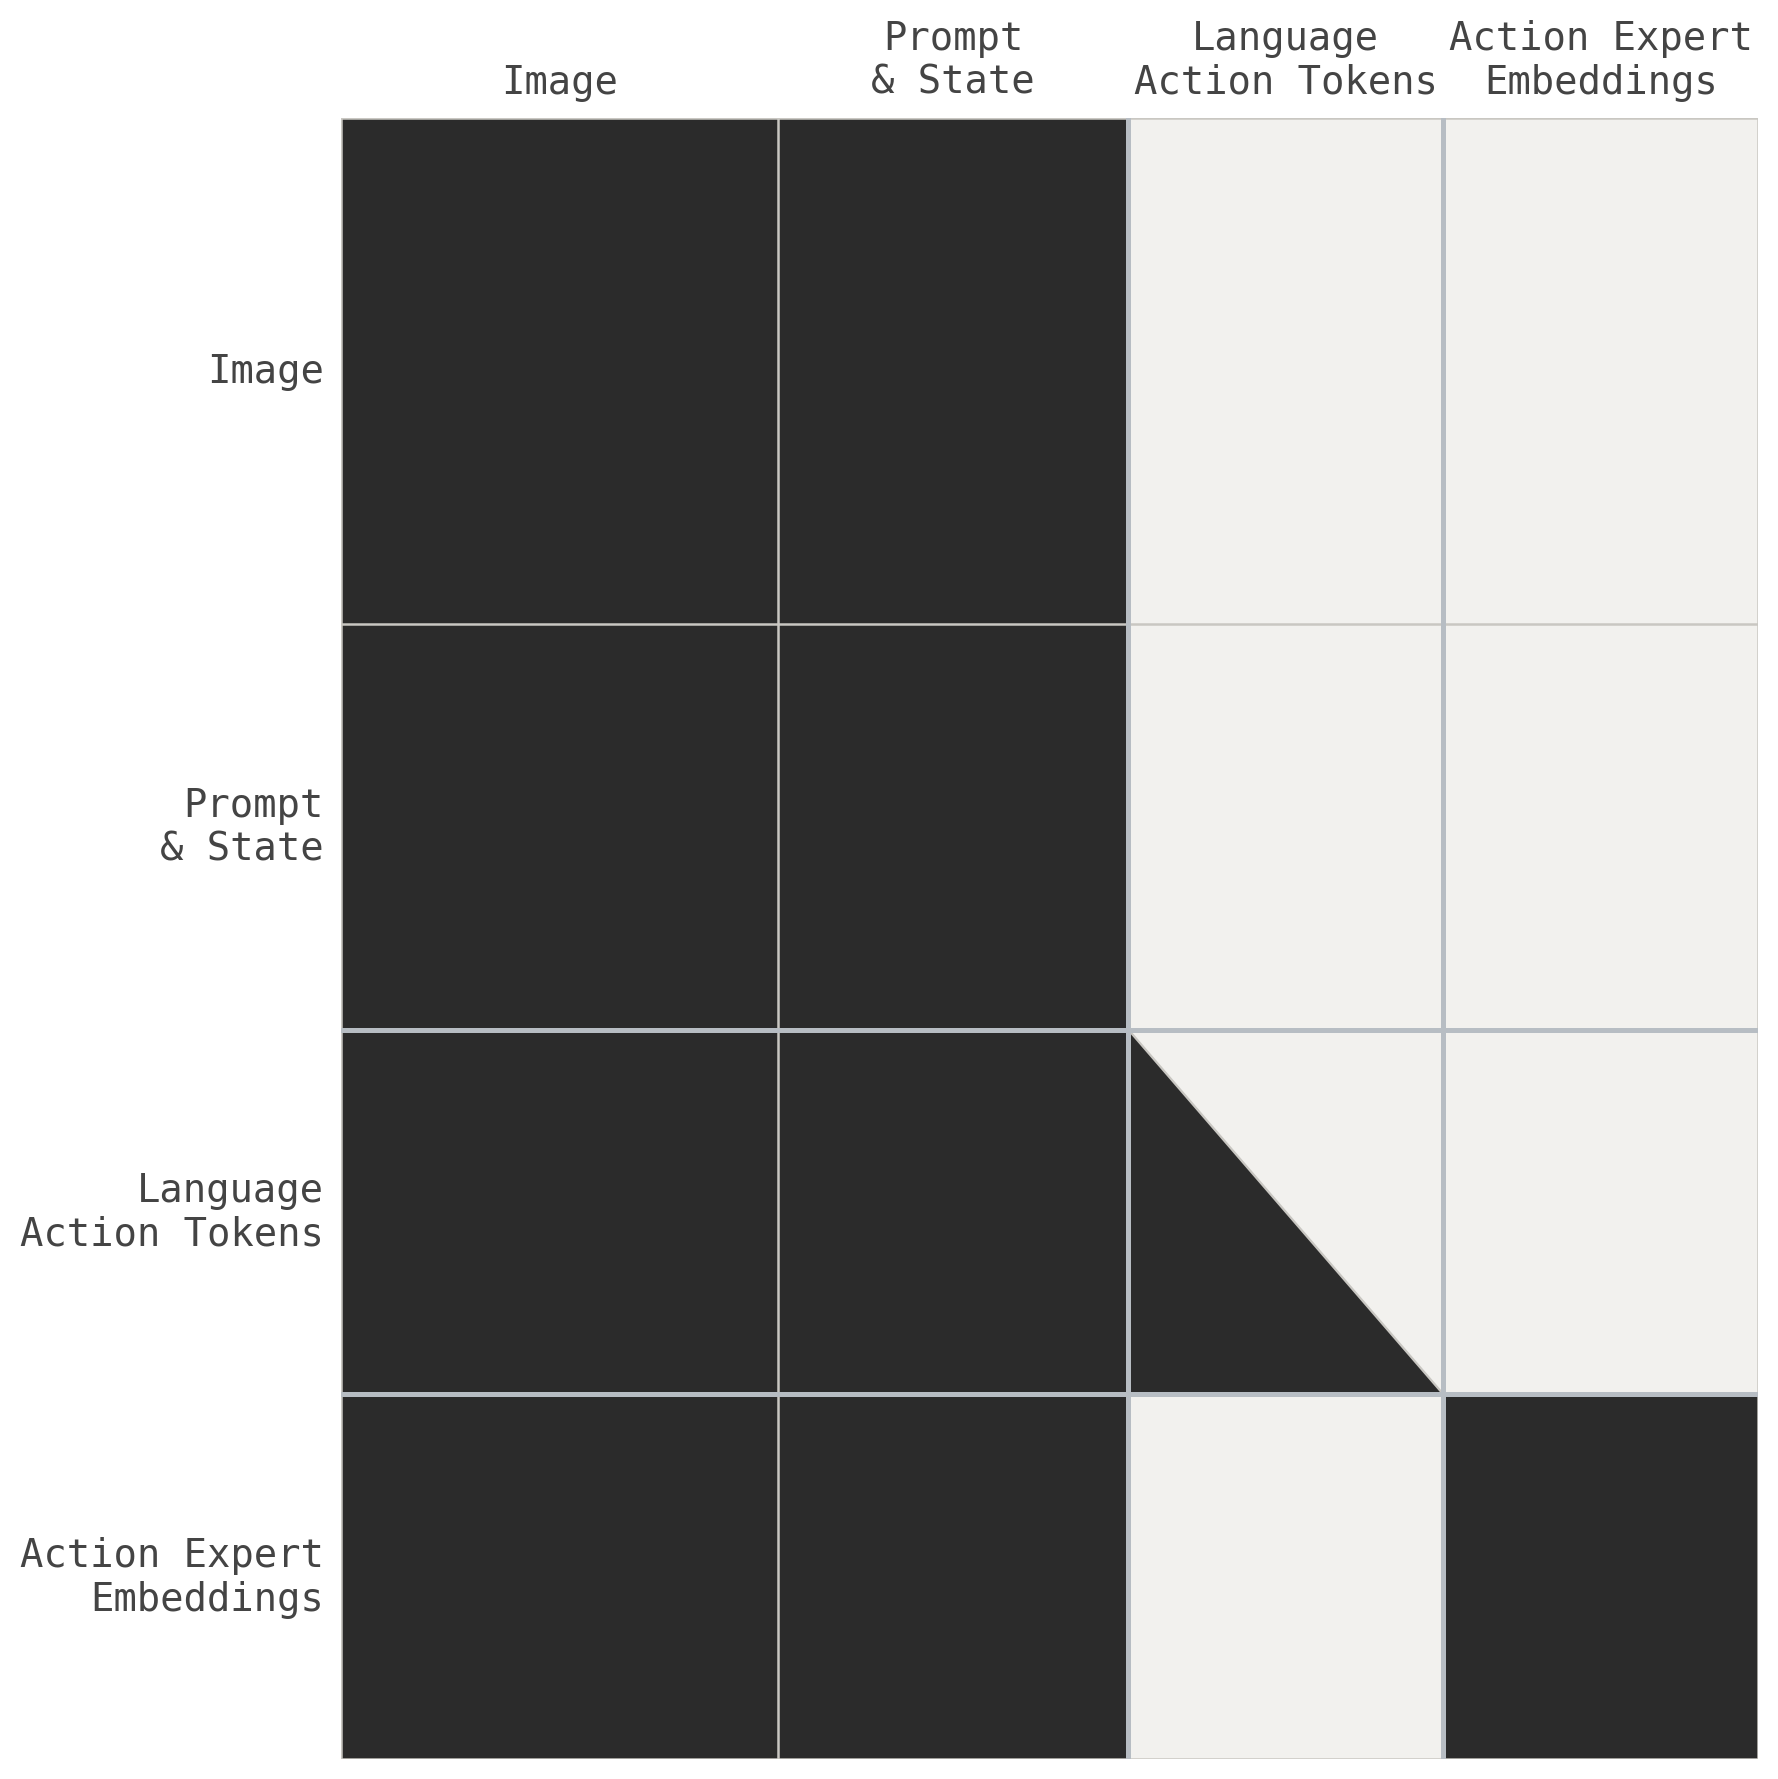
\includegraphics[width=\linewidth]{figures/appendix/fig10_attention_mask.png}
    \captionsetup{skip=3pt}
    \caption{Attention mask visualization for LAP-3B.}
    \label{fig:attention-mask}
    \vspace{-6pt}
\end{wrapfigure}
We visualize the attention mask of \textsc{LAP-3B} in Fig.~\ref{fig:attention-mask}. Prefix tokens—including image, prompt, and state—use bidirectional attention. Language-action tokens attend causally to one another while having full attention to all prefix tokens. The action expert uses full self-attention and fully attends to prefix tokens, but does not attend to language-action tokens.

\subsection{Flow-Matching Objective}
Given a ground-truth action chunk $a$ and base noise $z \sim \mathcal{N}(0,I)$, we construct an interpolated state
\[
x_\tau = (1-\tau)z + \tau a, \quad \tau \sim \mathcal{U}(0,1),
\]
with corresponding target velocity
\[
u = a - z .
\]
The action expert $v_\phi$ is trained via the flow-matching objective
\[
\mathcal{L}_{\text{flow}} =
\mathbb{E}\!\left[
\big\| v_\phi(x_\tau,\tau; o, l) - (a - z) \big\|_2^2
\right],
\]
which encourages the model to learn a continuous vector field transporting noise to valid actions conditioned on the observation and task.

At inference time, actions are generated by integrating the learned dynamics
\[
\frac{dx_\tau}{d\tau} = v_\phi(x_\tau,\tau; o, l)
\]
from $\tau=0$ to $\tau=1$ using a fixed-step explicit ODE solver.


\subsection{Training Data} 
The full dataset mixture used for training is summarized in Table~\ref{tab:data_mix}. The reported weights account for each dataset’s relative size and therefore reflect the true fraction of samples drawn from each source within a training batch. We assign a higher proportion to the DROID dataset~\cite{khazatsky2025droidlargescaleinthewildrobot} due to its broad task coverage and rich environmental diversity.

\begin{table}[th]
    \centering
    \caption{Training data mixture. Percentages denote the true fraction of samples from each dataset within each training batch.}
    
    \begin{tabular}{lr}
        \toprule
        \multicolumn{2}{c}{\textbf{Training Dataset Mixture}}\\
        \midrule
        DROID \cite{khazatsky2025droidlargescaleinthewildrobot} & 85.26\% \\
        Fractal \cite{brohan2023rt1roboticstransformerrealworld} & 5.86\% \\
        Bridge \cite{walke2024bridgedatav2datasetrobot} & 3.39\% \\
        BC-Z \cite{pmlr-v164-jang22a} & 0.47\% \\
        Taco Play \cite{mees2023groundinglanguagevisualaffordances} & 0.73\% \\
        Jaco Play \cite{dass2023jacoplay} & 0.12\% \\
        Furniture Bench Dataset \cite{heo2023furniturebenchreproduciblerealworldbenchmark} & 0.31\% \\
        UTAustin Mutex \cite{shah2023mutex} & 0.56\% \\
        Berkeley Fanuc Manipulation \cite{zhu2023fanuc} & 0.19\% \\
        FMB Dataset \cite{luo2024fmbfunctionalmanipulationbenchmark} & 0.09\% \\
        Berkeley Autolab UR5 \cite{BerkeleyUR5Website} & 0.15\% \\
        Austin Buds Dataset \cite{zhu2022bottomupskilldiscoveryunsegmented} & 0.05\% \\
        Austin Sailor Dataset \cite{nasiriany2022sailor} & 0.53\% \\
        Austin Sirius Dataset \cite{liu2023robotlearningjobhumanintheloop} & 0.44\% \\
        Viola \cite{zhu2023violaimitationlearningvisionbased} & 0.12\% \\
        MolmoAct \cite{lee2025molmoactactionreasoningmodels} & 1.73\% \\
        \bottomrule
    \end{tabular}
    \label{tab:data_mix}
\end{table}


During training, we filter idle segments by removing action sequences below a small motion threshold for consecutive steps and discard trajectories lacking task instructions.

\subsection{Compute and Infrastructure Details}
\label{app:compute}

\noindent\textbf{Hero-run compute.}
The final reported checkpoints for all models, including \textsc{LAP-3B}, \textsc{LAP-3B} with VQA co-training, and all replicated baselines, were trained using an identical large-scale pre-training setup. Each hero run was trained for approximately 50 hours on a TPU v6e-64 slice, corresponding to the checkpoints used for all main experiments. Across all reported models, the total hero-run compute amounts to approximately \textbf{50 TPU v6e-64 hours per model}.

\medskip
\noindent\textbf{Total pre-training compute.}
Across the full set of pre-training experiments—including \textsc{LAP-3B} and all replicated baselines, but excluding early prototyping, debugging runs, and downstream fine-tuning experiments—we conducted approximately 200 large-scale training runs. Collectively, these experiments consumed over \textbf{4,000 TPU v6e-64 hours}.

\medskip
\noindent\textbf{Inference compute.}
All real-robot evaluations are executed in real time using a single commodity GPU (an NVIDIA RTX 4090), without any additional model parallelism, specialized hardware, or acceleration techniques. End-to-end real-robot evaluation for the reported experiments required approximately \textbf{24 hours of total human-supervised runtime}.



\section{Evaluation Protocol}
\label{app:evaluation_details}

Each task is evaluated over 20 independent trials with randomized object placement within workspace bounds. A trial is terminated upon task success, time-out, or a safety-triggered abort, such as when the robot collides with the table, reaches joint limits, or exhibits unsafe behavior (e.g., excessively rapid or unstable motions).

For zero-shot experiments, we report binary task success along with 95\% finite-sample valid confidence intervals for binomial success rates, which control the Type-I error (miscoverage) probability \cite{vincent2024generalizablebehaviorcloningpolicy}.

For fine-tuning experiments, we use staged success scores to capture partial task completion:

\noindent$\bullet$ \emph{Hang Tape on Rack:}
\begin{itemize}
\item 0.25: reach the tape
\item 0.5: grasp the tape
\item 0.75: reach the rack while holding the tape
\item 1.0: successfully hang the tape
\end{itemize}

\noindent$\bullet$ \emph{Fold Towel and Place in Basket:}
\begin{itemize}
\item 0.5: correctly folded towel
\item 0.75: placed in basket but unfolded
\item 1.0: full task success
\end{itemize}




\begin{figure*}[t]
    \centering
    \includegraphics[width=\linewidth]{figures/appendix/fig9_rollout_visualization.pdf}
    \caption{\textbf{Zero-shot evaluation rollout visualizations.} Example observations from the camera views used for policy evaluation across different robot embodiments and tasks, shown from left to right.}
    \label{fig:zeroshot-rollout-visualization}
\end{figure*}

